%%%%%%%%%%%%%%%%%%%%%%%%%%%%%%%%%%%%%%%%%
% Masters/Doctoral Thesis 
% LaTeX Template
% Version 1.43 (17/5/14)
%
% This template has been downloaded from:
% http://www.LaTeXTemplates.com
%
% Original authors:
% Steven Gunn 
% http://users.ecs.soton.ac.uk/srg/softwaretools/document/templates/
% and
% Sunil Patel
% http://www.sunilpatel.co.uk/thesis-template/
%
% License:
% CC BY-NC-SA 3.0 (http://creativecommons.org/licenses/by-nc-sa/3.0/)
%
% Note:
% Make sure to edit document variables in the Thesis.cls file
%
%%%%%%%%%%%%%%%%%%%%%%%%%%%%%%%%%%%%%%%%%

%----------------------------------------------------------------------------------------
%	PACKAGES AND OTHER DOCUMENT CONFIGURATIONS
%----------------------------------------------------------------------------------------

\documentclass[11pt, oneside]{Thesis} % The default font size and one-sided printing (no margin offsets)

\graphicspath{{../graphics/}} % Specifies the directory where pictures are stored

\usepackage[square, numbers, comma, sort&compress]{natbib} % Use the natbib reference package - read up on this to edit the reference style; if you want text (e.g. Smith et al., 2012) for the in-text references (instead of numbers), remove 'numbers' 

%from my usual papers
\usepackage{amsmath}
\usepackage{amssymb}
\usepackage{amsthm}
\usepackage{amscd}
\usepackage{amsfonts}
\usepackage{graphicx}%
%\usepackage{fancyhdr}
%\usepackage{color}
%\usepackage{cite}
\usepackage{physics}
\usepackage{float}
\usepackage{caption}
\usepackage{subcaption}

\hypersetup{urlcolor=blue, colorlinks=true} % Colors hyperlinks in blue - change to black if annoying
\title{\ttitle} % Defines the thesis title - don't touch this

\begin{document}

\frontmatter % Use roman page numbering style (i, ii, iii, iv...) for the pre-content pages

\setstretch{1.3} % Line spacing of 1.3

% Define the page headers using the FancyHdr package and set up for one-sided printing
\fancyhead{} % Clears all page headers and footers
\rhead{\thepage} % Sets the right side header to show the page number
\lhead{} % Clears the left side page header

\pagestyle{fancy} % Finally, use the "fancy" page style to implement the FancyHdr headers

\newcommand{\HRule}{\rule{\linewidth}{0.5mm}} % New command to make the lines in the title page

%code handling
\newcommand{\raven}{\texttt{RAVEN}}
\newcommand{\bison}{\texttt{BISON}}
\newcommand{\moose}{\texttt{MOOSE}}

% some handy math stuff
\newcommand{\expv}[1]{\ensuremath{\mathbb{E}[ #1]}}
\newcommand{\xs}[2]{\ensuremath{\Sigma_{#1}^{(#2)}}}
\newcommand{\intO}{\ensuremath{\int\limits_{4\pi}}}
\newcommand{\intz}{\ensuremath{\int\limits_0^1}}
\newcommand{\intf}{\ensuremath{\int\limits_{-\infty}^\infty}}
\newcommand{\intzf}{\ensuremath{\int\limits_{0}^\infty}}
\newcommand{\LargerCdot}{\raisebox{-0.25ex}{\scalebox{1.2}{$\cdot$}}}
\newcommand{\hold}[1]{\ensuremath{\Big|_{#1}}}

\renewcommand{\vec}[1]{\mathbf{#1}}

% PDF meta-data
\hypersetup{pdftitle={\ttitle}}
\hypersetup{pdfsubject=\subjectname}
\hypersetup{pdfauthor=\authornames}
\hypersetup{pdfkeywords=\keywordnames}

%----------------------------------------------------------------------------------------
%	TITLE PAGE
%----------------------------------------------------------------------------------------

\begin{titlepage}
\begin{center}

\textsc{\LARGE \univname}\\[1.5cm] % University name
\textsc{\Large Doctoral Thesis}\\[0.5cm] % Thesis type

\HRule \\[0.4cm] % Horizontal line
{\huge \bfseries \ttitle}\\[0.4cm] % Thesis title
\HRule \\[1.5cm] % Horizontal line
 
\begin{minipage}{0.4\textwidth}
\begin{flushleft} \large
\emph{Author:}\\
%\href{http://www.johnsmith.com}
{\authornames} % Author name - remove the \href bracket to remove the link
\end{flushleft}
\end{minipage}
\begin{minipage}{0.4\textwidth}
\begin{flushright} \large
\emph{Supervisor:} \\
%\href{http://www.jamessmith.com}
{\supname} % Supervisor name - remove the \href bracket to remove the link  
\end{flushright}
\end{minipage}\\[3cm]
 
\large \textit{Submitted in partial fulfilment of the requirements\\ for the degree of \degreename}\\[0.3cm] % University requirement text
\textit{in the}\\[0.4cm]
%\groupname\\
\deptname\\[2cm] % Research group name and department name
 
{\large \today}\\[4cm] % Date
%\includegraphics{Logo} % University/department logo - uncomment to place it
 
\vfill
\end{center}

\end{titlepage}

%----------------------------------------------------------------------------------------
%	DECLARATION PAGE
%	Your institution may give you a different text to place here
%----------------------------------------------------------------------------------------

%\Declaration{
%
%\addtocontents{toc}{\vspace{1em}} % Add a gap in the Contents, for aesthetics
%
%I, \authornames, declare that this thesis titled, '\ttitle' and the work presented in it are my own. I confirm that:
%
%\begin{itemize} 
%\item[\tiny{$\blacksquare$}] This work was done wholly or mainly while in candidature for a research degree at this University.
%\item[\tiny{$\blacksquare$}] Where any part of this thesis has previously been submitted for a degree or any other qualification at this University or any other institution, this has been clearly stated.
%\item[\tiny{$\blacksquare$}] Where I have consulted the published work of others, this is always clearly attributed.
%\item[\tiny{$\blacksquare$}] Where I have quoted from the work of others, the source is always given. With the exception of such  quotations, this thesis is entirely my own work.
%\item[\tiny{$\blacksquare$}] I have acknowledged all main sources of help.
%\item[\tiny{$\blacksquare$}] Where the thesis is based on work done by myself jointly with others, I have made clear exactly what was done by others and what I have contributed myself.\\
%\end{itemize}
% 
%Signed:\\
%\rule[1em]{25em}{0.5pt} % This prints a line for the signature
% 
%Date:\\
%\rule[1em]{25em}{0.5pt} % This prints a line to write the date
%}

\clearpage % Start a new page

%----------------------------------------------------------------------------------------
%	QUOTATION PAGE
%----------------------------------------------------------------------------------------

\pagestyle{empty} % No headers or footers for the following pages

%\null\vfill % Add some space to move the quote down the page a bit
%
%\textit{``Thanks to my solid academic training, today I can write hundreds of words on virtually any topic without possessing a shred of information, which is how I got a good job in journalism."}
%
%\begin{flushright}
%Dave Barry
%\end{flushright}
%
%\vfill\vfill\vfill\vfill\vfill\vfill\null % Add some space at the bottom to position the quote just right
%
%\clearpage % Start a new page

%----------------------------------------------------------------------------------------
%	ABSTRACT PAGE
%----------------------------------------------------------------------------------------

\addtotoc{Abstract} % Add the "Abstract" page entry to the Contents

\abstract{\addtocontents{toc}{\vspace{1em}} % Add a gap in the Contents, for aesthetics

As the complexity of experiments in fields such as nuclear engineering continues to increase, so too does the
demand for robust computational methods to simulate these experiments in virtual space.  In many of these
simulations, exact input design parameters as well as intrinsic properties of the experiment are often sources
of input uncertainty.  Often, small perturbations in these uncertain parameters have significant impact on the
outcome of an experiment.  For instance, when considering nuclear fuel performance experiments, small changes
in the thermal conductivity of the fuel can greatly affect the maximum stress on the surrounding cladding.  In
recent years quantifying the impact of the input uncertainties in such an experimental system has grown as the
complexities in these systems increase.  For some problems, the input parametric space and corresponding
quantity of interest output space is sufficiently explored with a few low-cost computational calculations.
For others, however, the computational model is costly and it takes a great many random samples to obtain a
good understanding of the output space.  This research explores the possibilities of advanced methods in
stochastic collocation for generalized polynomial chaos (SCgPC) as an alternative to traditional uncertainty
quantification techniques such as Monte Carlo (MC) and Latin Hypercube sampling (LHS) methods.  In this
proposal we explore the behavior of traditional isotropic tensor product (TP) SCgPC, then expand to consider
truncated polynomial spaces using total degree (TD) and hyperbolic cross (HC) construction strategies.  Next,
we consider applying anisotropy to the polynomial space construction, and analyze methods whereby the level of
anisotropy can be approximated.  This leads to introducing the Sobol decomposition method, or high-dimensional
model representation (HDMR) method, both as a reduced-order model and as a method of obtaining sensitivity indices
for informing anisotropic SCgPC. We analyze these methods on nontrivial neutron diffusion transport problems.
Finally, we propose implementing adaptive algorithms for building both the polynomial space for SCgPC and the
constituent subset space of HDMR in order to approach ideal efficiency in modeling high-dimension problems.
Further, we propose implementing these methods in the uncertainty qunatification framework RAVEN and applying
them to nuclear fuels performance code BISON.
}

\clearpage % Start a new page

%----------------------------------------------------------------------------------------
%	ACKNOWLEDGEMENTS
%----------------------------------------------------------------------------------------

%\setstretch{1.3} % Reset the line-spacing to 1.3 for body text (if it has changed)
%
%\acknowledgements{\addtocontents{toc}{\vspace{1em}} % Add a gap in the Contents, for aesthetics
%
%The acknowledgements and the people to thank go here, don't forget to include your project advisor\ldots
%}
%\clearpage % Start a new page

%----------------------------------------------------------------------------------------
%	LIST OF CONTENTS/FIGURES/TABLES PAGES
%----------------------------------------------------------------------------------------

\pagestyle{fancy} % The page style headers have been "empty" all this time, now use the "fancy" headers as defined before to bring them back

\lhead{\emph{Contents}} % Set the left side page header to "Contents"
\tableofcontents % Write out the Table of Contents

\lhead{\emph{List of Figures}} % Set the left side page header to "List of Figures"
\listoffigures % Write out the List of Figures

\lhead{\emph{List of Tables}} % Set the left side page header to "List of Tables"
\listoftables % Write out the List of Tables

%----------------------------------------------------------------------------------------
%	ABBREVIATIONS
%----------------------------------------------------------------------------------------

%\clearpage % Start a new page
%
%\setstretch{1.5} % Set the line spacing to 1.5, this makes the following tables easier to read
%
%\lhead{\emph{Abbreviations}} % Set the left side page header to "Abbreviations"
%\listofsymbols{ll} % Include a list of Abbreviations (a table of two columns)
%{
%\textbf{LAH} & \textbf{L}ist \textbf{A}bbreviations \textbf{H}ere \\
%%\textbf{Acronym} & \textbf{W}hat (it) \textbf{S}tands \textbf{F}or \\
%}
%
%%----------------------------------------------------------------------------------------
%%	PHYSICAL CONSTANTS/OTHER DEFINITIONS
%%----------------------------------------------------------------------------------------
%
%\clearpage % Start a new page
%
%\lhead{\emph{Physical Constants}} % Set the left side page header to "Physical Constants"
%
%\listofconstants{lrcl} % Include a list of Physical Constants (a four column table)
%{
%Speed of Light & $c$ & $=$ & $2.997\ 924\ 58\times10^{8}\ \mbox{ms}^{-\mbox{s}}$ (exact)\\
%% Constant Name & Symbol & = & Constant Value (with units) \\
%}
%
%%----------------------------------------------------------------------------------------
%%	SYMBOLS
%%----------------------------------------------------------------------------------------
%
%\clearpage % Start a new page
%
%\lhead{\emph{Symbols}} % Set the left side page header to "Symbols"
%
%\listofnomenclature{lll} % Include a list of Symbols (a three column table)
%{
%$a$ & distance & m \\
%$P$ & power & W (Js$^{-1}$) \\
%% Symbol & Name & Unit \\
%
%& & \\ % Gap to separate the Roman symbols from the Greek
%
%$\omega$ & angular frequency & rads$^{-1}$ \\
%% Symbol & Name & Unit \\
%}
%
%%----------------------------------------------------------------------------------------
%%	DEDICATION
%%----------------------------------------------------------------------------------------
%
%\setstretch{1.3} % Return the line spacing back to 1.3
%
%\pagestyle{empty} % Page style needs to be empty for this page
%
%\dedicatory{For/Dedicated to/To my\ldots} % Dedication text
%
%\addtocontents{toc}{\vspace{2em}} % Add a gap in the Contents, for aesthetics

%----------------------------------------------------------------------------------------
%	THESIS CONTENT - CHAPTERS
%----------------------------------------------------------------------------------------

\mainmatter % Begin numeric (1,2,3...) page numbering

\pagestyle{fancy} % Return the page headers back to the "fancy" style

% Include the chapters of the thesis as separate files from the Chapters folder
% Uncomment the lines as you write the chapters

% Chapter 1

\chapter{Introduction} % Main chapter title

\label{Chapter1} % For referencing the chapter elsewhere, use \ref{Chapter1} 

\lhead{1. \emph{Introduction}} % This is for the header on each page - perhaps a shortened title

%----------------------------------------------------------------------------------------

%\section{Welcome and Thank You}

%problem description
Fuels performance codes are numerical simulations intended to characterize the performance of a set of
materials in a particular geometry under a certain environment, over time.  The environmental considerations
might include temperature, neutron flux, external pressure, and similar factors.  In many cases, the
performance is quantified by considering the maximum stress undergone by cladding around the fuel as it
expands and makes contact.  By varying the construction materials and geometry of the fuel, its cladding, and
the gap between them, fuel can be designed for optimal performance without experiencing a rupture or similar
break.

%introduce uq for problem
There are a plethora of parameters that go into simulating fuel performance.  The fuel itself is made up of
many constituent materials with a variety of densities and structures, as well as behavior under irradiation.
The contents of the fuel-cladding gap determine how effectively heat can conduct out of the fuel and to the
cladding, then out to a moderator, and the thickness of this gap determines the amount of fuel expansion
allowed before contact is made and outward pressure begins increasing.  The material and geometry of the
cladding determine limits on stress and efficiency of heat transfer.  Any of the material properties in the
fuel, gap, or cladding, along with the environmental conditions, can be a source of uncertainty in determining
the maximum stress applied to the cladding.

%explain nature of uncertainty
There are two categories into which sources of uncertainty fall: aleatoric, or the statistical uncertainty inherent in a
system; and epistemic, or the systematic uncertainty due to imprecision in measurement or existence of
measurable unknowns.  While there are aleatoric uncertainties in fuel performance (such as the neutronics of
irradiated fuel), in this work we consider mostly epistemic uncertainties surrounding the material properties
and geometries of the problems.  For an example case, we can consider the overall reactor power, fuel mesoscale
grain growth, and fuel thermal expansion coefficient as uncertain input parameters, with maximum Von Mises stress in the 
axial center of a fuel rod as a quantity of interest in the output space.

%explain scope of proposal
In this work, we consider several methodologies for quantifying the uncertainty in fuel performance
calculations.  In order to demonstrate clearly the function of these methods, we demonstrate them first on
several simpler problems, such as polynomial evaluations or projectile motion.  The first method we consider
is traditional, analog Monte Carlo (MC) analysis, wherein random sampling of the input space generates a view of
the output space.  MC is used as a benchmark methodology; if other methods converge on quantities of interest
more quickly and accurately than MC, we consider them ``better'' for our purposes.

The second method we consider is isotropic, tensor-product (TP) stochastic collocation for generalized polynomial
chaos (SCgPC)\cite{sparseSC}\cite{sparse1}\cite{sparse2}\cite{xiu}, whereby deterministic collocation points are used to develop a polynomial reduced-order model
of the output quantities of interest as a function of the inputs.  The other methods we consider expand on
this method.  First, we introduce non-tensor-product methods for determining polynomial bases, using the 
total degree (TD) and hyperbolic cross (HC) polynomial set construction methods\cite{hctd}.
These bases will then be used to construct Smolyak-like sparse grids for collocation\cite{smolyak}.  Second, we consider
anisotropic sparse grids,
allowing additional collocation points for preferential input parameters.  We also consider methods for
determining weights that determine the level of preference to give parameters, and explore the effects of a
variety of anisotropic choices.

The third method we consider is high-dimension model representation (HDMR), which correlates with Sobol
decomposition \cite{hdmr}.  This method is useful both for developing sensitivities of the quantity of interest to subsets
of the input space, as well as constructing a reduced-order model itself.  We demonstrate the strength of HDMR
as a method to inform anisotropic sensitivity weights for SCgPC.

Additionally, we propose continued work on developing adaptive algorithms for both SCgPC and HDMR\cite{Ayres}.  In adaptive
SCgPC, the polynomial basis is constructed level-by-level based on the highest-impact subset polynomials.  In
adaptive HDMR, the constituent subset input spaces are developed similarly, based on the highest-impact input
subset.  The crowning achievement we propose is combining HDMR and SCgPC to develop both the subset input
space as well as the overall reduced-order model adaptively in an attempt to construct a
competitively-efficient method for uncertainty quantification.

Finally, we propose all these methods be developed within Idaho National Laboratory's \raven{}\cite{raven}
uncertainty quantification framework. \raven{} is a Python-written framework that non-intrusively provides
tools for analysts to quantify the uncertainty in their simulations with minimal impact. \raven{}  has already
been shown to work seamlessly with \moose{}-based fuel performance code \bison{}\cite{moose}\cite{bison}, on which we propose to demonstrate the various
methods described above.

%outline chapters
The remainder of this work will proceed as follows:
\begin{itemize}
  \item Chapter 2: We mathematically describe the problems solved by the simulations we will be running,
    including polynomial evaluations, attenuation, projectile, diffusion, and fuel performance.  We discuss
    their potential applications and approach using random sampling.
  \item Chapter 3: We describe our implementation of SCgPC, including isotropic and anisotropic, as well as
    TP, TD, and HC construction strategies.
  \item Chapter 4: We describe our implementation of HDMR, and its possible applications as both a
    reduced-order model and a method for determining sensitivity coefficients.
  \item Chapter 5: We discuss proposed work extending both SCgPC and HDMR to be constructed adaptively.  We
    also discuss the predicted shortfalls in the adaptive algorithms and some potential methods to address
    them.
\end{itemize}
%----------------------------------------------------------------------------------------

% Chapter Template

\chapter{Simulation Physics} % Main chapter title

\label{Chapter2} % Change X to a consecutive number; for referencing this chapter elsewhere, use \ref{ChapterX}

\lhead{Chapter 2. \emph{Simulation Physics}} % Change X to a consecutive number; this is for the header on each page - perhaps a shortened title

%----------------------------------------------------------------------------------------
%	SECTION 1
%----------------------------------------------------------------------------------------

\section{Simulations Used}
To demonstrate the efficacy of the various uncertainty quantification methods we use in this work, we employ
several independent simulations (hereafter referred to as ``codes'') of increasing complexity.  These codes
range from simple polynomial evaluations to analytic solutions of simple physics, to nonlinear multistage
iterative solvers representing complex codes.  We describe each briefly here.

\section{Polynomial Evaluations}
In order to benchmark the simplest cases, we make use of simple polynomial expressions of the form
\begin{equation}
  u(Y) = \prod_{i=1}^N (y^b_i+a),
\end{equation}
where $u(Y)$ is the quantity of interest, $Y=[y_1,y_2,\ldots,y_N]$ is the vector of uncertain inputs, and $a$
and $b$ are arbitrary scalar values.  The input variables $Y$ can be distributed arbitrarily.
These polynomials are demonstrations where SCgPC evaluates exactly at some
finite expansion level.




\section{Attenuation}
To demonstrate the convergence rates of various methods, we make use of an adjusted attenuation problem that
is equivalent to the penetration of point particles in a purely-absorbing medium.  The uncertain input
variables are each the length of a segment of material, and each segment has an identical cross section equal
to 1.  The quantity of
interest is the percentage of particles exiting the material.  We normalize the length of the segments to
preserve significant values for the percentage exiting.  The solution to this problem is
\begin{align}
  u(Y) &= \prod_{i=1}^N e^{-Y_i/L},\\
  u(Y) &= \sum_{i=1}^N \exp\left[\frac{\sum_{i=1}^N -Y_i}{L}\right],
\end{align}
where $L=|Y|_1$ is the total segment length.  The input variables $Y$ can be distributed arbitrarily.

The benefit of this model is a simple analytic solution, which makes analytic benchmarks possible.  In
addition, because of the exponential form, SCgPC will converge on a solution, but not replicate it exactly as
in the polynomial case.  This allows accurate comparison between MC, SCgPC methods, and HDMR methods.




\section{Projectile}
For a nonlinear case without an analytic solution, we consider the path traveled by a projectile near the
surface of the Earth, considering varying gravitational pull with height as well as drag on the projectile
from stagnant air.  The equations governing travel in both vertical position $x$ and horizontal position $y$
are given by
\begin{equation}
  y(t) = \frac{v_T}{g}(v\sin\theta+v_T)\left(1-\exp\left[\frac{-gt}{v_T}\right]\right)-v_T t,
\end{equation}
\begin{equation}
  x(t) = \frac{vv_T\cos\theta}{g}\left(1-\exp\left[\frac{-gt}{v_T}\right]\right),
\end{equation}
where $t$ is time, $g$ is acceleration due to gravity, $v$ is scalar velocity, $\theta$ the angle between the
velocity vector and the horizontal ground, $v_T=\frac{mg}{D}$ is terminal velocity, $D=\frac{\rho CA}{2}$ is
the acceleration due to drag, $C$ is the drag coefficient, and $A=\pi r^2$
is the surface area of the projectile in the direction of travel.  The projectile is assumed to present an
identical surface area in both $x$ and $y$ directions.  The quantity of interest is the range, or the total
distance in $x$ traveled by the ball before reaching a height of $y=0$.  The uncertain input variables are
distributed uniformly as described in Table \ref{tab:proj dist}.

\begin{table}[h]
\centering
\begin{tabular}{c | l | c c | c}
  Variable & Name & Mean & Range ($\pm$) & Units \\\hline
  $y_i$ & Initial Height & 1 & 1 & m\\
  $v$ & Initial Velocity & 35.5 & 2.5 & m/s\\
  $\theta$ & Initial Angle & 45 & 10 & degrees\\
  $g$ & Accel. Gravity & 9.79888 & 0.0349 & m/s/s\\
  $m$ & Projectile Mass & 0.145 & 0.0725 & kg\\
  $r$ & Projectile Radius & 0.0336 & 0.00336 & m\\
  $C$ & Drag Coefficient & 0.5 & 0.5 & \\
  $\rho$ & Air Density & 1.2 & 0.1 & kg/m$^3$ \\
\end{tabular}
\caption{Projectile Problem Distributions}
\label{tab:proj dist}
\end{table}

This simulation has the benefit of an analytic solution when $C=0$ and eight distinct input parameters of
varying importance.  This is especially useful in considering anisotropic treatment of the input space.




\section{Neutron Diffusion}
For a nonlinear system with complicated physics, we consider a two-group, two-dimensional neutron diffusion
criticality calculation.  We make use of the diffusion approximation for neutron transport, which provides us
with a coupled set of elliptic PDEs to solve:
\begin{equation}
-\grad\cdot\qty( D_1(\bar x)\grad\phi_1(\bar x))+\qty(\xs{a}{1}(\bar x)+\xs{s}{1\to2}(\bar x))\phi_1(\bar x) = \frac{1}{k(\phi)}\sum_{g'=1}^2\nu_{g'}\xs{f}{g'}(\bar x)\phi_{g'}(\bar x),
\end{equation}
\begin{equation}
-\grad \cdot\qty(D_2(\bar x)\grad \phi_2(\bar x))+\xs{a}{2}(\bar x)\phi_2(\bar x) = \xs{s}{1\to 2}(\bar x)\phi_1(\bar x),
\end{equation}
where we use the following parametric coefficients: the absorption cross section
$\Sigma_{g,a}=\Sigma_{g,c}+\Sigma_{g,f}$; the capture and fission cross sections $\Sigma_{g,c}$ and
$\Sigma_{g,f}$; the diffusion coefficient $D_g$ which depends on the scattering cross section of the medium;
and the fission multiplication factor $\nu_g$, the ratio of new neutrons per fission-producing neutron.  The
solution to this PDE is the neutron scalar flux $\phi_g(\bar x)$.  We apply no-traction conditions on the
vacuum boundaries and zero-derivative current on the reflecting boundaries for both energy groups:
\begin{equation}
\frac{\phi_g}{4}-\frac{D_g}{2}\eval{\pdv{\phi_g}{x_1}}_{\partial \Omega_\text{top}}=0,\hspace{5pt} g=1,2,
\end{equation}
\begin{equation}
\frac{\phi_g}{4}-\frac{D_g}{2}\eval{\pdv{\phi_g}{x_2}}_{\partial \Omega_\text{right}}=0,\hspace{5pt} g=1,2,
\end{equation}
\begin{equation}
-D_g\eval{\pdv{\phi_g}{x_1}}_{\partial \Omega_\text{bottom}}=0,\hspace{5pt} g=1,2,
\end{equation}
\begin{equation}
-D_g\eval{\pdv{\phi_g}{x_2}}_{\partial \Omega_\text{left}}=0,\hspace{5pt} g=1,2.
\end{equation}
\\
The criticality eigenvalue and quantity of interest $k(\phi)$ is given by
\begin{equation}
k(\phi)=\sum_{g=1}^2\iint\limits_D\frac{\nu\xs{f}{g}\phi_g(\bar x)}{\qty(-\nabla\cdot D_g\nabla+\Sigma_r^{(g)})\phi_g(\bar x)}~d\bar x.
\end{equation}
We address solving $\phi_1,\phi_2,$ and $k$ nonlinearly and simultaneously.  
The material properties are shown in Table \ref{tab:coremats}, and the domain $\Omega=[0,200\text{ cm}]^2$.
The reference flux solutions are plotted in Fig. \ref{benchflux}, and for the reference problem
$k$=1.00007605445.  \begin{figure}[H]
\centering
  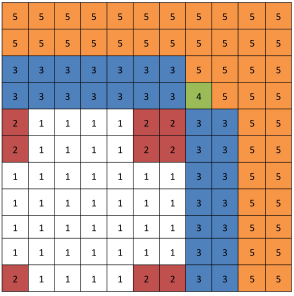
\includegraphics[width=0.4\linewidth]{core}
  \caption{Core Geometry}
  \label{geom}
\end{figure}
\begin{table}[h]
\centering
\begin{tabular}{c c | c c c c}
Region & Group & $D_g$ & $\Sigma_{a,g}$ & $\nu\Sigma_{f,g}$ & $\Sigma_s^{1,2}$ \\ \hline
1 & 1 & 1.255 & 8.252e-3 & 4.602e-3 & 2.533e-2 \\
 & 2 & 2.11e-1 & 1.003e-1 & 1.091e-1 & \\ \hline
2 & 1 & 1.268 & 7.181e-3 & 4.609e-3 & 2.767e-2 \\
 & 2 & 1.902e-1 & 7.047e-2 & 8.675e-2 & \\ \hline
3 & 1 & 1.259 & 8.002e-3 & 4.663e-3 & 2.617e-2 \\
 & 2 & 2.091e-1 & 8.344e-2 & 1.021e-1 & \\ \hline
4 & 1 & 1.259 & 8.002e-3 & 4.663e-3 & 2.617e-2 \\
 & 2 & 2.091e-1 & 7.3324e-2 & 1.021e-1 & \\ \hline
5 & 1 & 1.257 & 6.034e-4 & 0 & 4.754e-2 \\
 & 2 & 1.592e-1 & 1.911e-2 & 0 & 
\end{tabular}
\caption{Reference Material Properties for Benchmark Core}
\label{tab:coremats}
\end{table}
\begin{figure}[H]
\centering
  \begin{subfigure}[b]{0.45 \textwidth}
   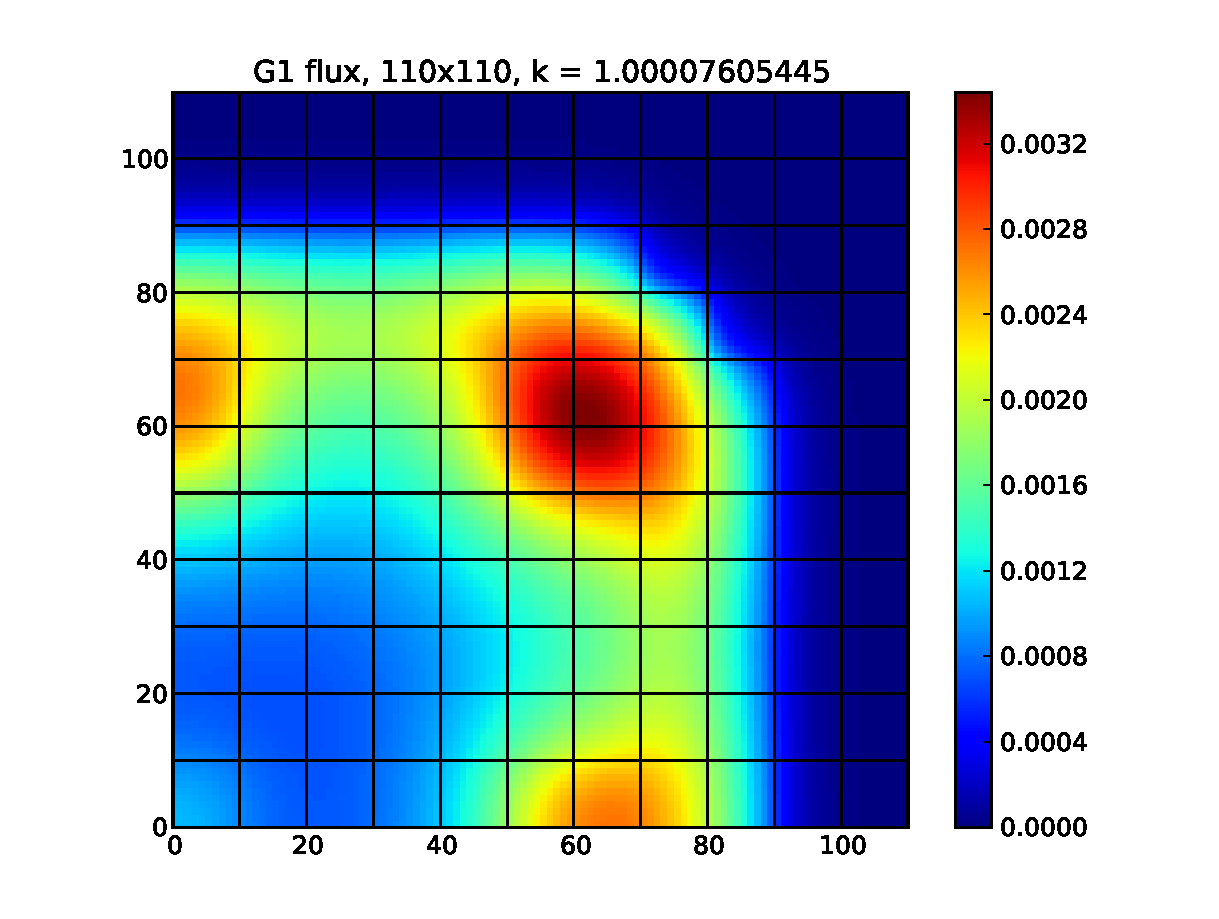
\includegraphics[width=\textwidth]{g1_50_flux}
   \caption{$\phi$, Group 1}
   \label{g1}
  \end{subfigure}
  \begin{subfigure}[b]{0.45 \textwidth}
   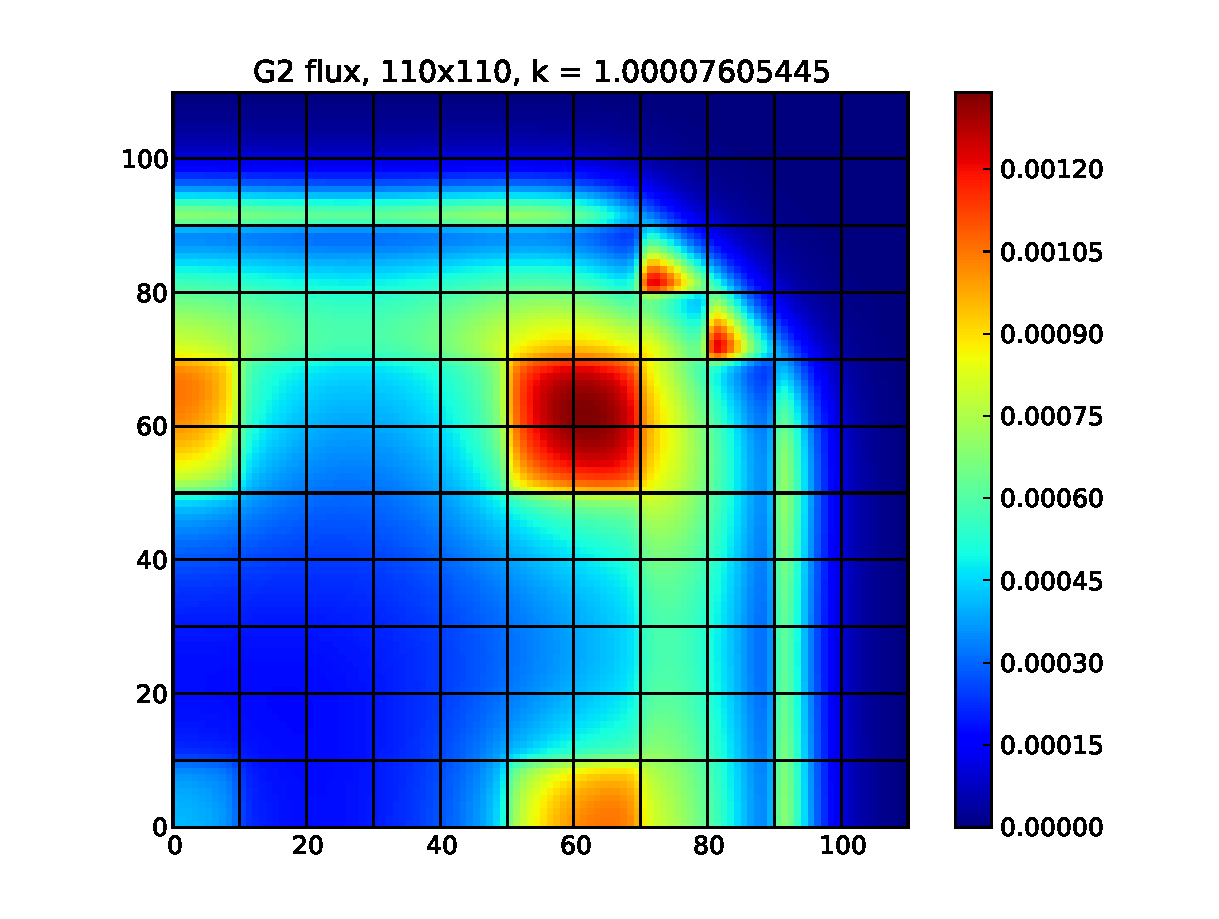
\includegraphics[width=\textwidth]{g2_50_flux}
   \caption{$\phi$, Group 2}
   \label{g2}
  \end{subfigure}
  \caption{Reference Flux Profiles}
  \label{benchflux}
\end{figure}



\section{Fuel Rod Performance}
While the previous codes were designed and written by the author, \bison{} is a professional use code
maintained by Idaho National Laboratory.  The fuel performance simulation used in this work is described
in \cite{cristiansmeared},
and involves an axial-symmetric LWR fuel rodlet, composed of ten uranium dioxide pellets, zirconium-4
cladding, gap, and upper plenum.  The problem is a power ramp-up transient as delineated in Table
\ref{tab:bison power ramp}.  The three uncertain input parameters are distributed in a truncated normal and
are shown in Table \ref{tab:bison dists}.  Note that scaling parameters are used for both grain radius and
reactor power, such that a scaling factor of one is the nominal unperturbed case.
\begin{table}[h]
  \centering
  \begin{tabular}{c|c}
    Time (s) & Linear Power (W/m) \\ \hline
    0 & 0 \\
    1e4 & 3.5e4 \\
    1.5e8 & 3.5e4
  \end{tabular}
  \caption{Linear Power Time Evolution}
  \label{tab:bison power ramp}
\end{table}
\begin{table}[h]
  \centering
  \begin{tabular}{c|c|c}
    Variable & Min. Value & Max. Value \\ \hline
    Grain Radius Scale Factor & 0.4 & 1.5 \\
    Thermal Expansion Coefficient & 9e-6 & 1.1e-5 \\
    Linear Power Scaling Factor & 0.95 & 1.05
  \end{tabular}
  \caption{Fuel Performance Input Distributions}
  \label{tab:bison dists}
\end{table}

The quantity of interest are the stresses on the axial center of the cladding.  The
uncertain parameters used in this test case are the mesoscale grain radius of the fuel, the simulated power
of the reactor surrounding the fuel rod, and the thermal expansion coefficient of the fuel.
 
% Chapter Template

\chapter{Stochastic Collocation and generalized Polynomial Chaos} % Main chapter title

\label{Chapter3} % Change X to a consecutive number; for referencing this chapter elsewhere, use \ref{ChapterX}

\lhead{Chapter 3. \emph{SC and gPC}} % Change X to a consecutive number; this is for the header on each page - perhaps a shortened title

%----------------------------------------------------------------------------------------
%	SECTION 1
%----------------------------------------------------------------------------------------

\section{Uncertainty Quantification Methods}
We consider a few methods for uncertainty quantification (UQ).  One method to classify UQ methods is by their
interaction level with a simulation code.  Non-intrusive methods treat the code as a black box, perturbing the
inputs and collecting the outputs without modifying the code.  These methods are ideal for generic application
frameworks, where the simulation code may be unknown or precompiled.  Examples of non-intrusive methods
include analog Monte Carlo (MC), Latin Hypercube sampling (LHS), and deterministic collocation methods.
Alternatively, intrusive methods require access to the solution algorithm itself.  Sometimes this can provide
more efficient solutions.  In particular, adjoint methods require the solution operator to be reversible, and
provide very efficient methods to determine sensitivities and analyze output-input dependence.  While many
intrusive methods have benefits, they lack the flexibility and universal applicability of non-intrusive
methods, and so we neglect them in this work.

\section{Correlation}
An assumption we make going forward is that the uncertain input parameters are independent or at least
uncorrelated.  If this is not the case, methods such as Karhunen-Loeve expansion can be used to develop an orthogonal
input space to replace the original.  Similarly, principle component analysis can be used to attempt to find
the fundamental uncorrelated space that maps into the correlated variable space.

\section{Monte Carlo}
In analog Monte Carlo uncertainty quantification, a single point in the input space is selected randomly,
and an output collected, until an appropriately accurate view of the output space is acquired.  While few
samples result in a poor understanding of the quantity of interest, sufficiently large samples converge on a
correct solution.  The convergence rate of Monte Carlo is consistent, as
\begin{equation}
  \epsilon = \frac{c}{\sqrt{\eta}},
\end{equation}
where $c$ is a constant and $\eta$ is the number of samples taken.  While this convergence rate is slow, it is possibly one of the
most reliable methods available.  This makes MC a good choice for benchmarking.

One of the downsides of MC (and LHS) when compared with other methods is that they do not generate a
reduced-order model as part of the evaluation; however, interpolation methods can be used to generate
additional samples.

\section{Latin Hypercube Sampling}
Latin hypercube sampling\cite{lhs} is another stochastic method that specializes in multidimensional
distributions.  In this method

% Chapter Template

\chapter{Proposed Work} % Main chapter title

\label{Chapter4} % Change X to a consecutive number; for referencing this chapter elsewhere, use \ref{ChapterX}

\lhead{Chapter 4. \emph{Proposed Work}} % Change X to a consecutive number; this is for the header on each page - perhaps a shortened title

%----------------------------------------------------------------------------------------
%	SECTION 1
%----------------------------------------------------------------------------------------

\section{Proposal}
There are several opportunities to continue this preliminary work.  First, it is possible \cite{Gerstner} to
adaptively construct polynomial index sets instead of using deterministic index sets.  Similarly, HDMR can be
expanded with adaptive algorithms to build up the representation in consecutive subsets\cite{Ayres}.  These adaptive
algorithms have been shown to greatly affect the curse of dimensionality, to the point where HDMR based on
SCgPC is competitive with Monte Carlo sampling for input spaces with dimensionality on the order of hundreds.

In concert with this, while Gaussian quadrature is effective at integrating polynomials, it has been shown
\cite{goodclenshaw} that other quadratures with convenient properties can compete effectively with them.  In
particular, when performing adaptive sampling, nested quadratures offer a significant reduction in necessary
computational cost for convergence, since quadrature points are re-used in successive layers.  We propose
implementing and considering some nested quadrature strategies such as Clenshaw-Curtis and Gauss-Patterson and
analyzing their impact on convergence when used in SCgPC.

Similarly, it would be of interest to contrast the use of Lagrange polynomials in the gPC expansion with
versus the Wiener-Askey polynomials used thus far.  We expect to see little change in convergence rates except
in cases where the simulation model is easily-replicated by either set of polynomial families.

Lastly, we propose implementing all the methods described in this work in the \raven{} uncertainty
quantification framework, and perform thorough analysis on a selected \bison{} case.  Similar analysis has
been performed recently \cite{bigbison} but without the benefit of some of the adaptive and combined
strategies established and proposed in this work.  Such implementation would demonstrate significant viability
for the methods and make them more readily available to uncertainty quantification analysts.
 
%\input{Chapters/Chapter5} 
%\input{Chapters/Chapter6} 

%----------------------------------------------------------------------------------------
%	THESIS CONTENT - APPENDICES
%----------------------------------------------------------------------------------------

%\addtocontents{toc}{\vspace{2em}} % Add a gap in the Contents, for aesthetics

%\appendix % Cue to tell LaTeX that the following 'chapters' are Appendices

% Include the appendices of the thesis as separate files from the Appendices folder
% Uncomment the lines as you write the Appendices

%% Appendix A

\chapter{Appendix Title Here} % Main appendix title

\label{AppendixA} % For referencing this appendix elsewhere, use \ref{AppendixA}

\lhead{Appendix A. \emph{Appendix Title Here}} % This is for the header on each page - perhaps a shortened title

Write your Appendix content here.
%\input{Appendices/AppendixB}
%\input{Appendices/AppendixC}

%\addtocontents{toc}{\vspace{2em}} % Add a gap in the Contents, for aesthetics

\backmatter

%----------------------------------------------------------------------------------------
%	BIBLIOGRAPHY
%----------------------------------------------------------------------------------------

\label{Bibliography}

\lhead{\emph{Bibliography}} % Change the page header to say "Bibliography"

\bibliographystyle{unsrtnat} % Use the "unsrtnat" BibTeX style for formatting the Bibliography

\bibliography{Bibliography} % The references (bibliography) information are stored in the file named "Bibliography.bib"

\end{document}
